
\section{Langkah-Langkah Percobaan}

\subsection{Crimping Kabel LAN}

\begin{enumerate}
  \item Sebelum memulai praktikum, diberikan modul untuk melakukan crimping yang berisi: kabel LAN (belum jadi), kepala LAN (RJ45), cutter, tang potong, dan alat crimping.
  \item Crimping kabel dilakukan dengan cara memotong ujung kabel dan mengekspos isi kabel di dalamnya 
  \item Kabel-kabel tersebut diurai dan diurutkan sesuai dengan standar warna, seperti pada gambar berikut:

  \begin{figure}[H]
    \centering
    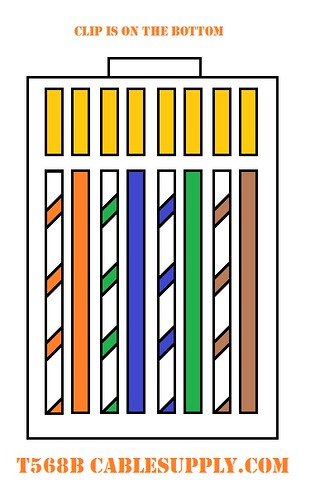
\includegraphics[width=0.2\linewidth]{P1/img/2.jpg}
    \caption{Urutan Warna Kabel LAN}
    \label{fig:inirujukan}
  \end{figure}

  \item Setelah diurutkan, kabel dipotong secara simetris menggunakan alat crimping.
  \item Kabel yang sudah rapi dan terurut dimasukkan ke dalam kepala RJ45.
  \item Kepala RJ45 yang telah berisi kabel kemudian dimasukkan ke dalam alat crimping dan ditekan sampai terdengar bunyi klik.
  \item Lakukan langkah yang sama pada sisi kabel lainnya, sehingga satu kabel memiliki dua ujung RJ45.
  \item Masukkan kedua ujung kabel ke dalam LAN Cable Tester.
  \item Jika semua LED pada tester menyala secara berurutan, maka proses crimping berhasil.
\end{enumerate}

\subsection{Routing IPv4 Menggunakan Router Statis}

\begin{enumerate}
  \item Pastikan router dalam keadaan default (reset) agar konfigurasi tidak mengalami konflik.
  \item Gunakan aplikasi Winbox untuk login ke router via MAC Address. Username default adalah \texttt{admin}, tanpa password.
  \item {Konfigurasi IP Address Antar Router:}
  \begin{itemize}
    \item Router 1 (ether1): \texttt{10.10.10.1/30}
    \item Router 2 (ether1): \texttt{10.10.10.2/30}
  \end{itemize}
  \item {Konfigurasi IP Address untuk Jaringan LAN:}
  \begin{itemize}
    \item Router 1 (ether2): \texttt{192.168.10.1/27}
    \item Router 2 (ether2): \texttt{192.168.20.1/27}
  \end{itemize}
  \item {Tambahkan Routing Statis:}
  \begin{itemize}
    \item Di Router 1:
    \begin{itemize}
      \item \texttt{Dst. Address: 192.168.20.0/27}
      \item \texttt{Gateway: 10.10.10.2}
    \end{itemize}
    \item Di Router 2:
    \begin{itemize}
      \item \texttt{Dst. Address: 192.168.10.0/27}
      \item \texttt{Gateway: 10.10.10.1}
    \end{itemize}
  \end{itemize}
  \item {Konfigurasi IP Address pada Laptop:}
  \begin{itemize}
    \item Laptop 1:
    \begin{itemize}
      \item IP: \texttt{192.168.10.2}
      \item Netmask: \texttt{255.255.255.224}
      \item Gateway: \texttt{192.168.10.1}
    \end{itemize}
    \item Laptop 2:
    \begin{itemize}
      \item IP: \texttt{192.168.20.2}
      \item Netmask: \texttt{255.255.255.224}
      \item Gateway: \texttt{192.168.20.1}
    \end{itemize}
  \end{itemize}
  \item {Pengujian Koneksi:} Lakukan \texttt{ping} dari Laptop 1 ke Laptop 2. Jika reply diterima, maka routing berhasil.
  \item {Catatan:} Jika koneksi gagal, pastikan firewall dalam keadaan nonaktif.
\end{enumerate}

\subsection{Routing IPv4 Menggunakan Router Dinamis}
Tahap ini kosong, karena saat melakukan praktikum kelompok kami tidak berhasil melakukan routing statis.



\section{Analisis Hasil Percobaan}
Pada percobaan crimping, kami mempelajari bahwa, kabel lan akan dapat bekerja dengan baik apabila, kabel-kabel kecil didalamnya di urutkan sesuai dengan warna yang seharusnya. Panjang kabel yang keluar dari kepala RJ45 juga menentukan apakah kabel tersebut akan bertahan lama.  

Pada Percobaan routing statis bertujuan menghubungkan dua jaringan agar bisa saling berkomunikasi melalui router. Secara teori, hal ini dilakukan dengan memberikan IP address dan menambahkan rute secara manual.

Namun, saat pengujian konektivitas, tidak ada respons yang diterima. Kemungkinan besar kesalahan terjadi pada pengisian IP address atau gateway yang tidak sesuai. Karena waktu terbatas, kami tidak sempat memperbaiki konfigurasi dan melanjutkan ke percobaan routing dinamis.


\section{Hasil Tugas Modul}
\begin{enumerate}
    \item Soal:\\ Berdasarkan tugas pendahuluan sebelumnya mengenai perancangan topologi jaringan dan tabel IP yang telah Anda buat, langkah selanjutnya adalah membuat simulasi jaringan menggunakan aplikasi Cisco Packet Tracer. Silakan lakukan konfigurasi pada masing-masing perangkat agar seluruh jaringan dapat saling terhubung dan berkomunikasi dengan baik.
\\ Jawab: 
\begin{figure}[H]
    \centering
    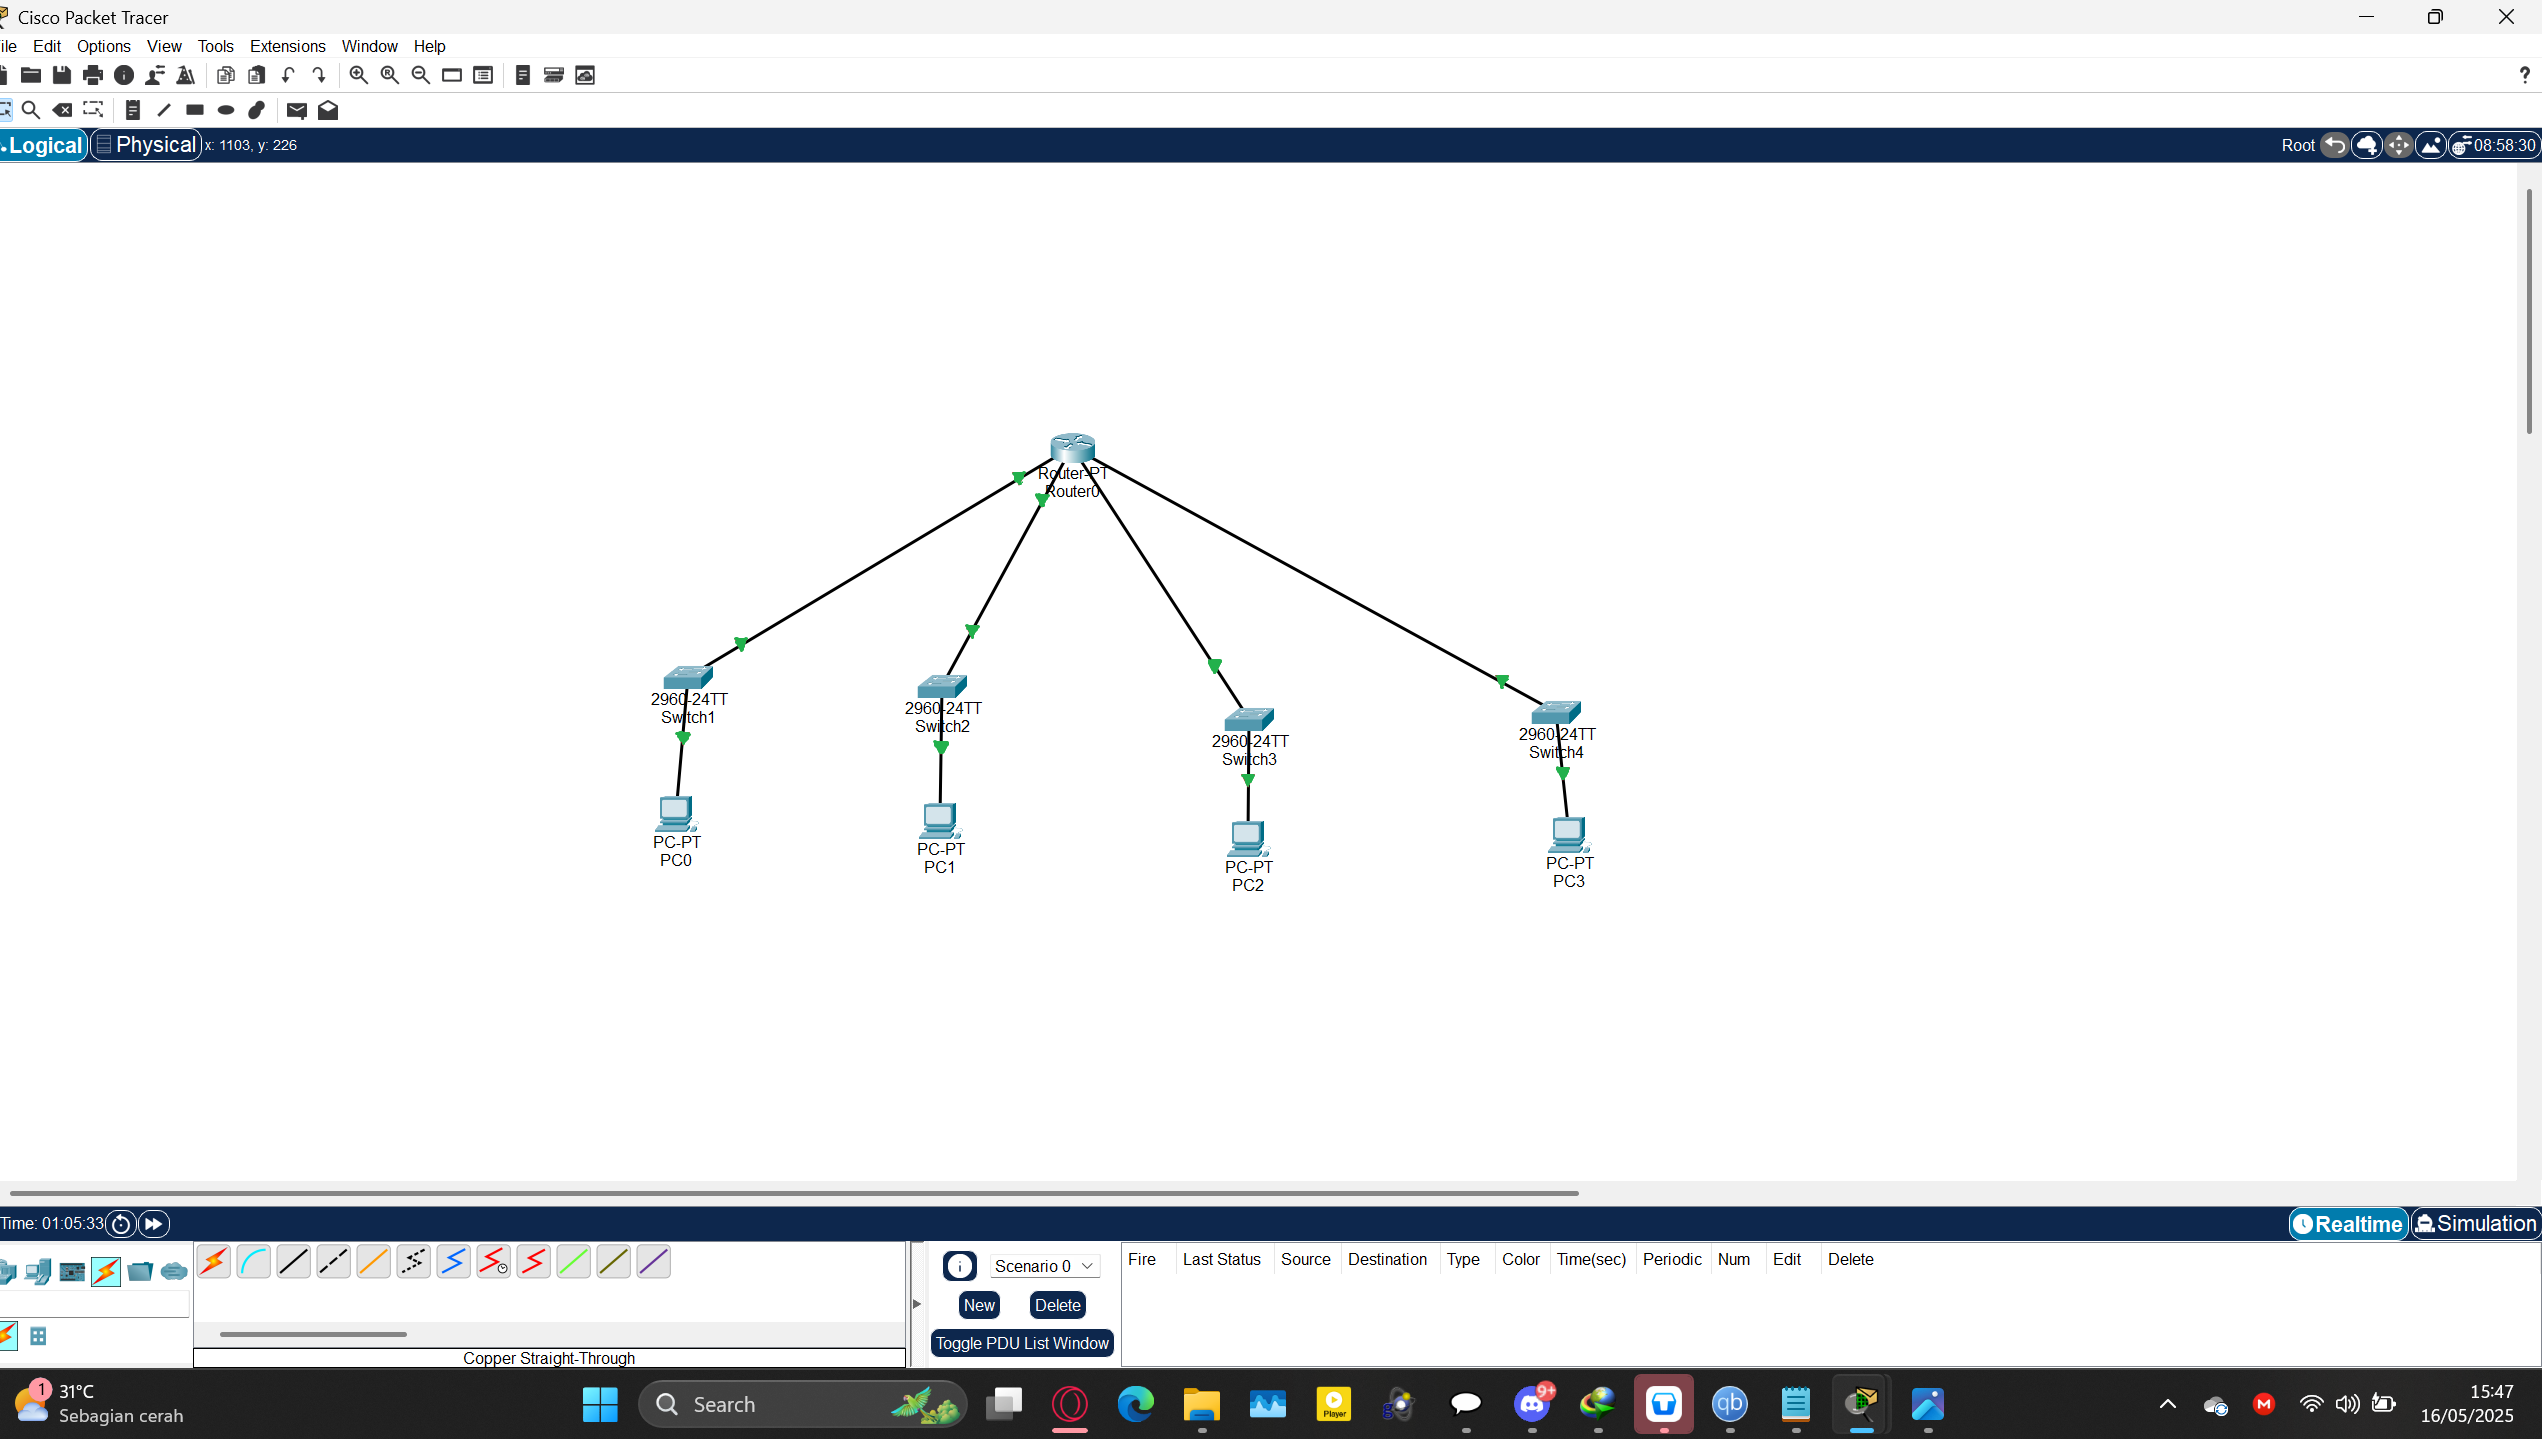
\includegraphics[width=1\linewidth]{P1/img/3.png}
    \caption{Urutan Warna Kabel LAN}
    \label{fig:inirujukan}
  \end{figure}

\item Soal: \\ Jelaskan apa kesulitan yang anda alami pada Praktikum.
\\Jawab: \\
Selama praktikum, kami mengalami beberapa kendala, terutama pas bagian routing statis. Awalnya kami kira sudah paham dari penjelasan teori, tapi saat mencobanya langsung ternyata masih bingung. Kemungkinan ada kesalahan se-waktu mengisi IP atau netmask, jadi koneksi antar laptop nggak jalan.Waktunya yang terbatas, jadi kami tidak sempat ngecek satu-satu konfigurasinya. Karena itu, bagian routing dinamis pun belum sempat kami kerjakan.Selain itu, beberapa dari kami juga baru pertama kali pakai Mikrotik dan Winbox. Jadi saat melihat tampilannya, butuh waktu buat adaptasi dan mencari yang dibutuhkan.

\end{enumerate}

\section{Kesimpulan}
Berdasarkan praktikum yang sudah di lakukan dapat diambil kesimpulan bahwa, kabel LAN memiliki urutan yang harus diikuti agar dapat berjalan dengan baik, dan dapat kita ketahui dari pengujian menggunakan tester. Pada bagian routing statis, kami mencoba menghubungkan dua jaringan menggunakan router MikroTik. Meskipun secara teori routing statis cukup sederhana, hasil praktik menunjukkan bahwa konfigurasi IP dan routing harus dilakukan dengan sangat teliti. Sayangnya, hasil yang kami dapat belum sesuai dengan teori karena terjadi kesalahan konfigurasi dan keterbatasan waktu.

\section{Lampiran}
\subsection{Dokumentasi saat praktikum}

\begin{figure}[H]
    \centering
    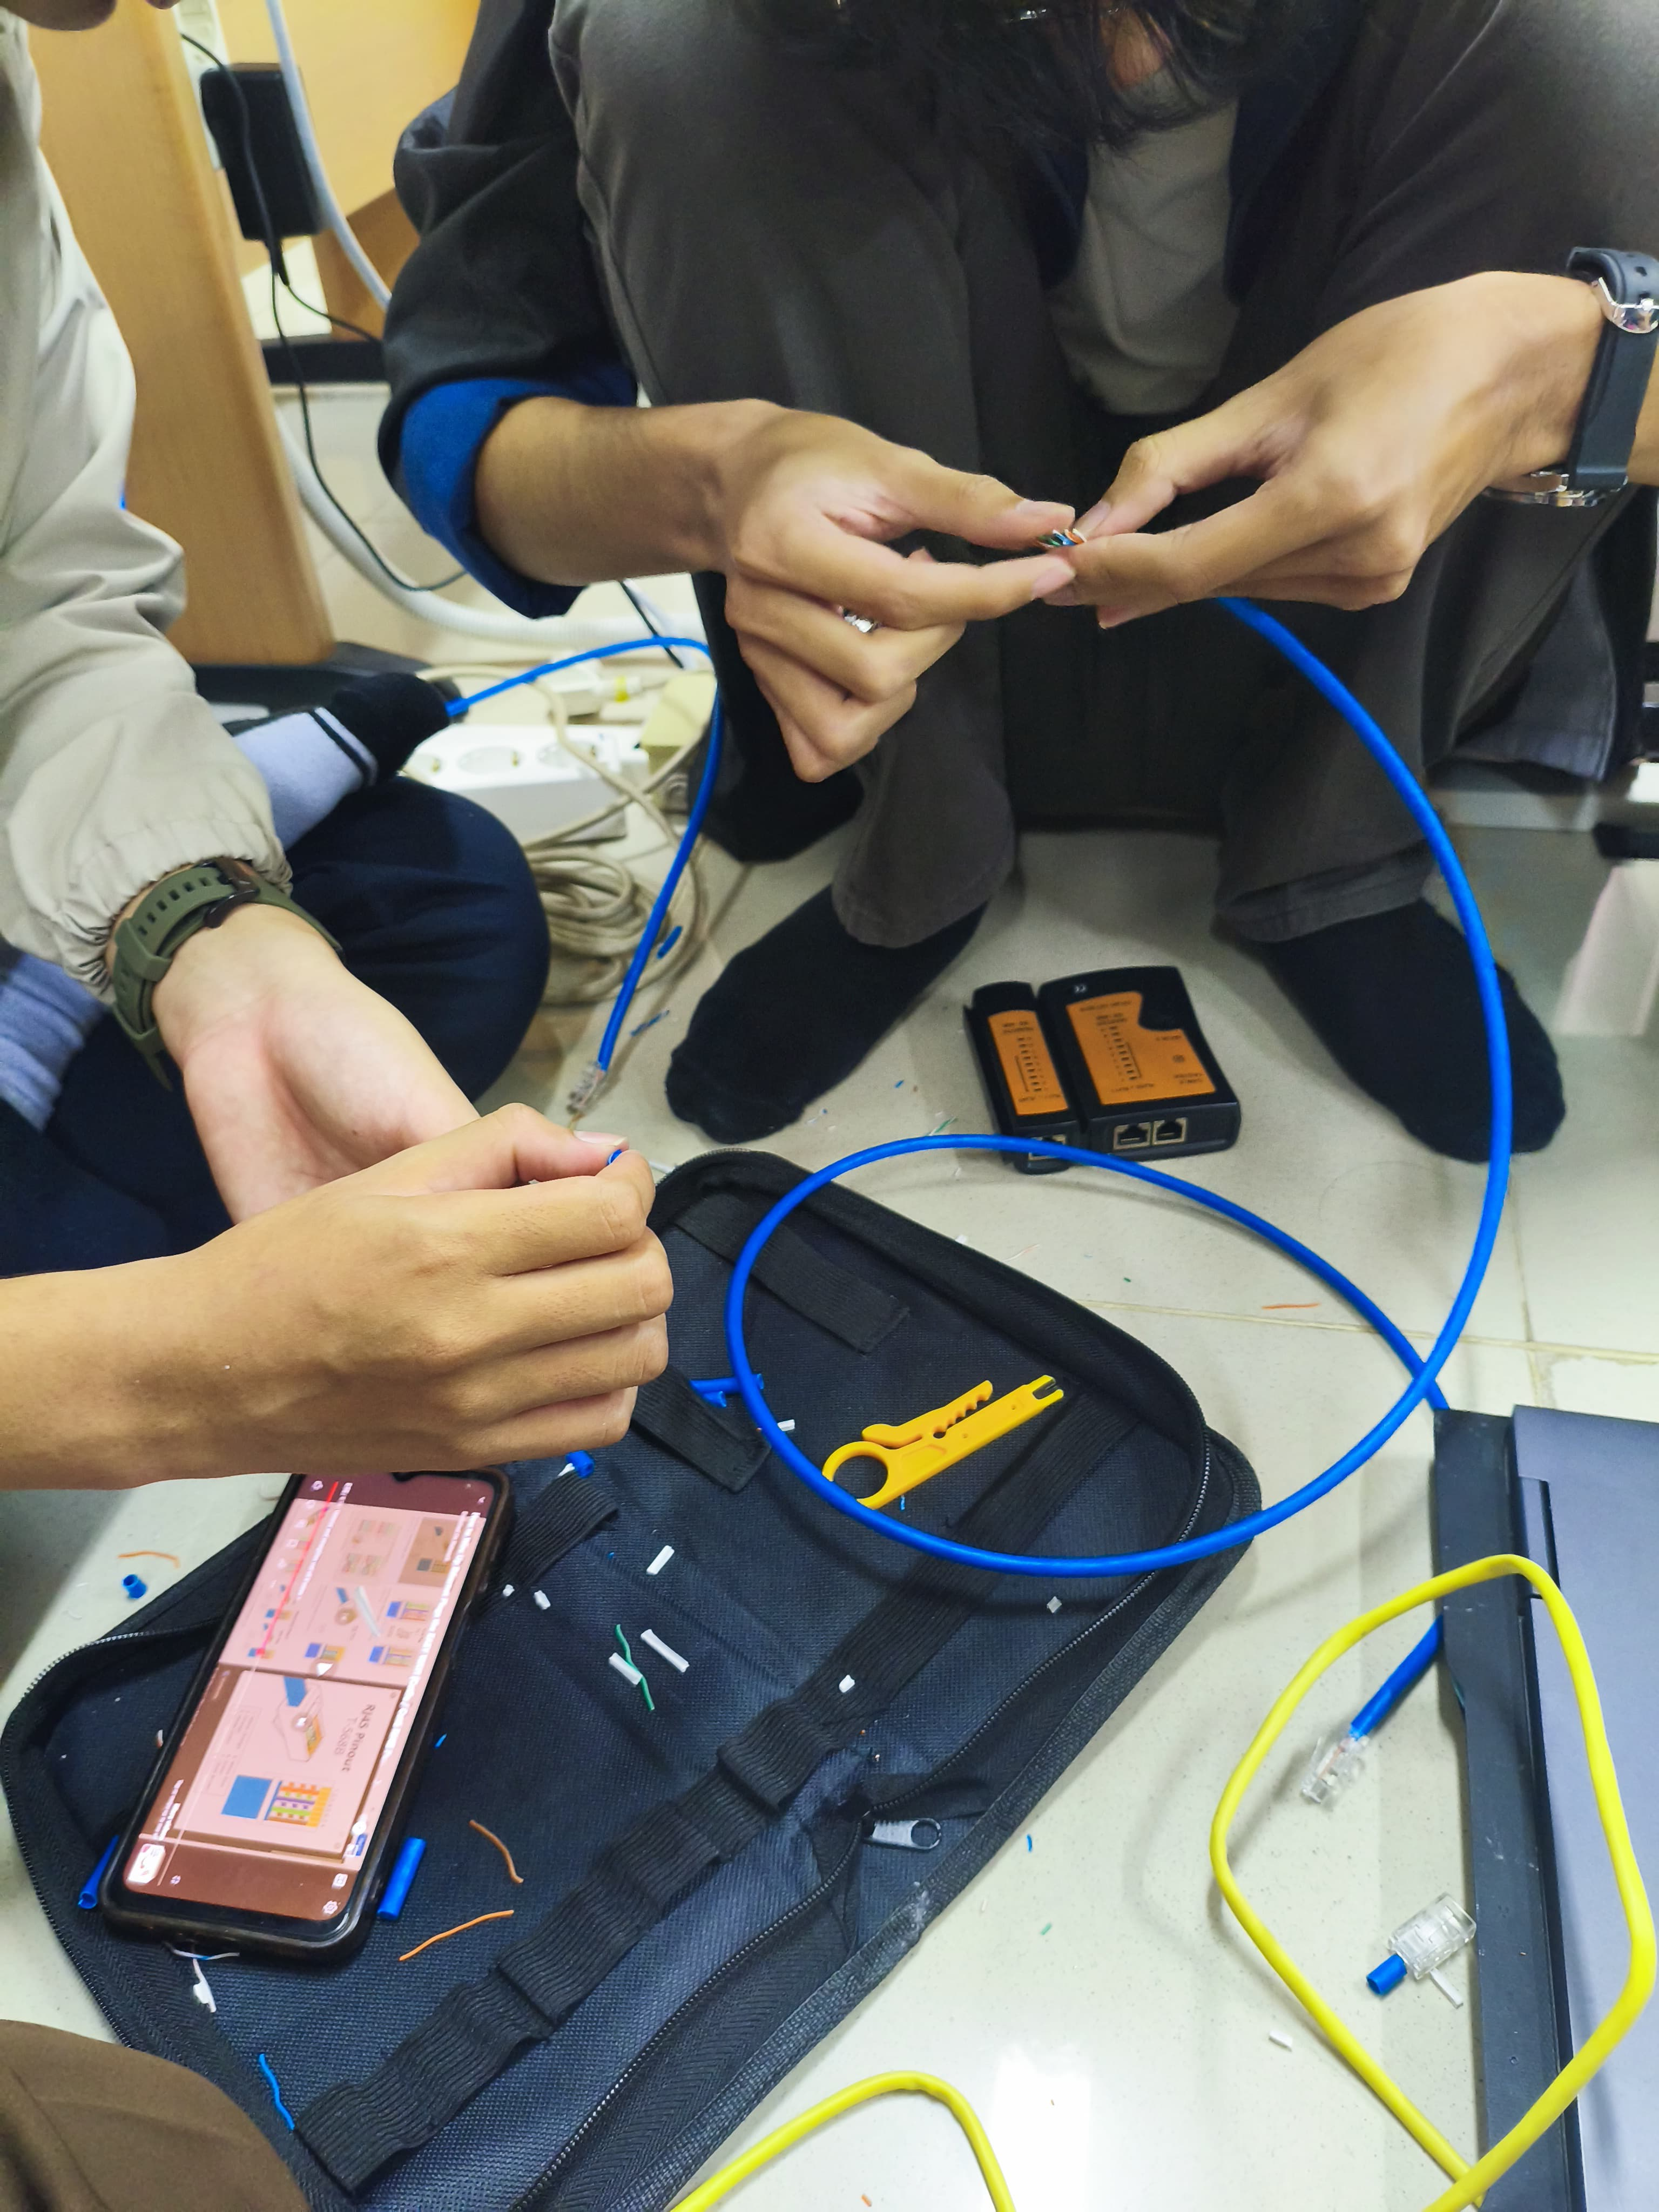
\includegraphics[width=0.5\linewidth]{P1/img/4.jpeg}
    \caption{Ketika melakukan Crimping}
    \label{fig:inirujukan}
  \end{figure}
  
\begin{figure}[H]
    \centering
    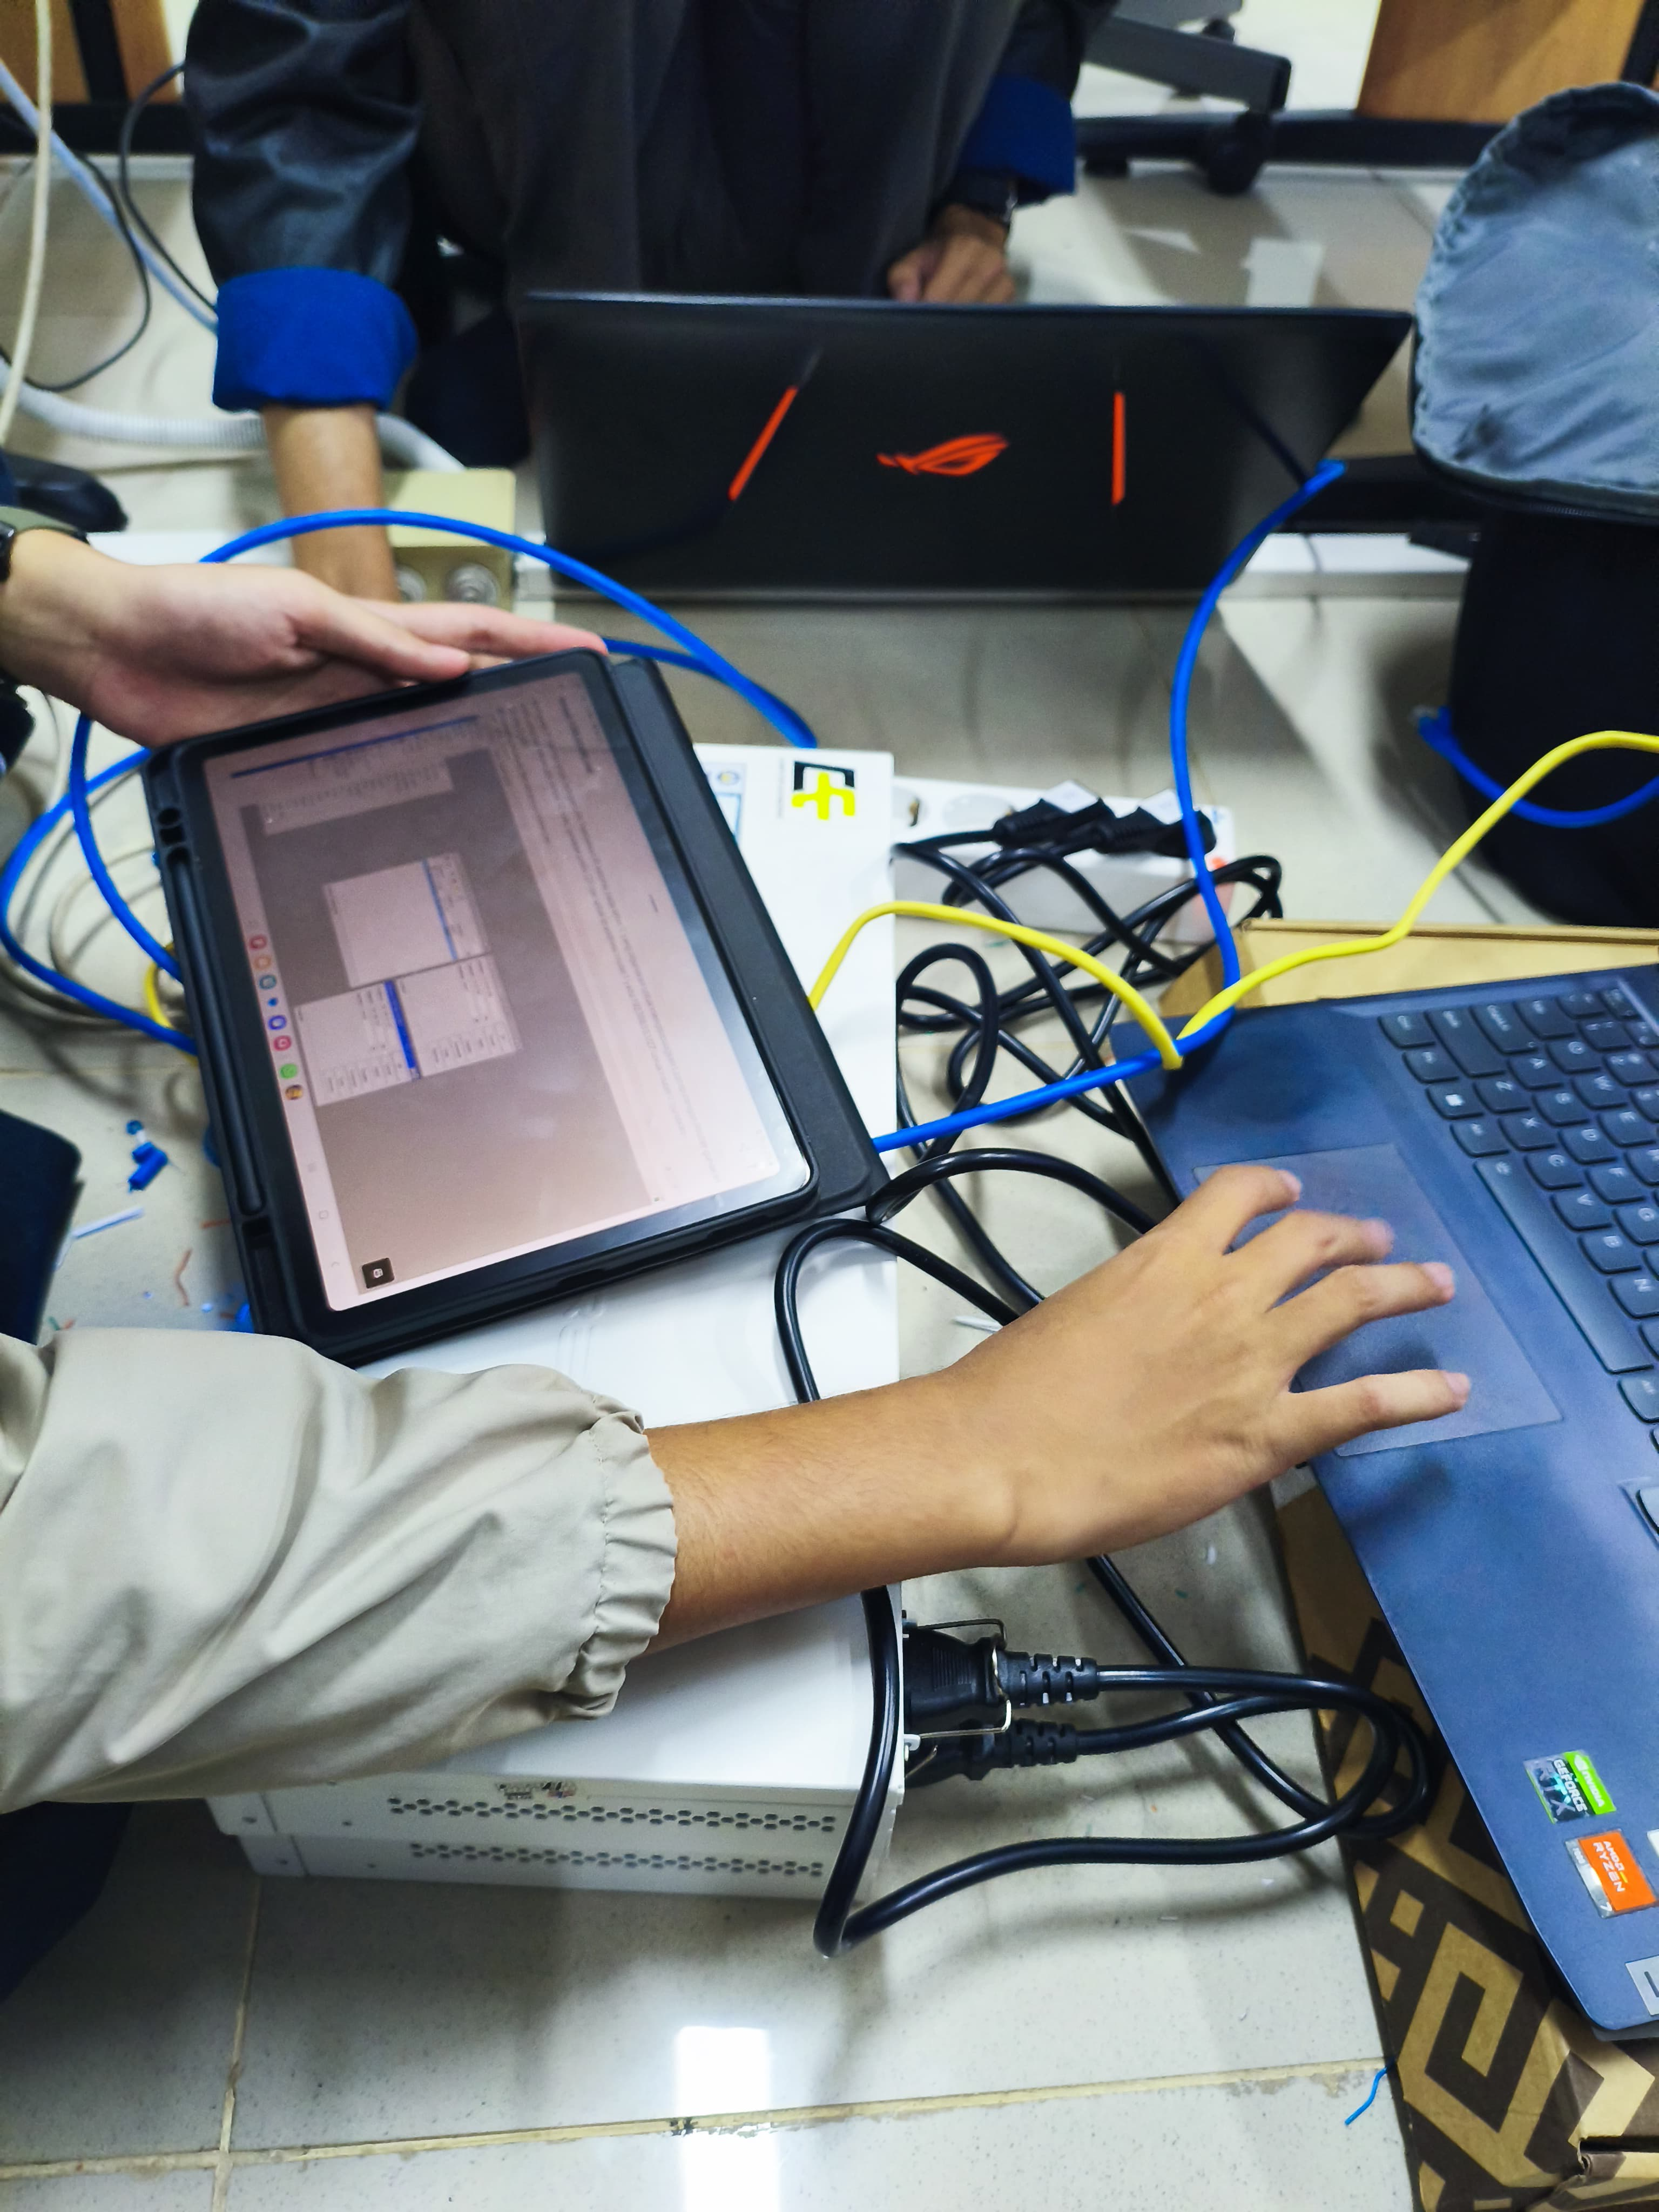
\includegraphics[width=0.5\linewidth]{P1/img/5.jpeg}
    \caption{Saat melakukan Routing}
    \label{fig:inirujukan}
  \end{figure}

  \begin{figure}[H]
    \centering
    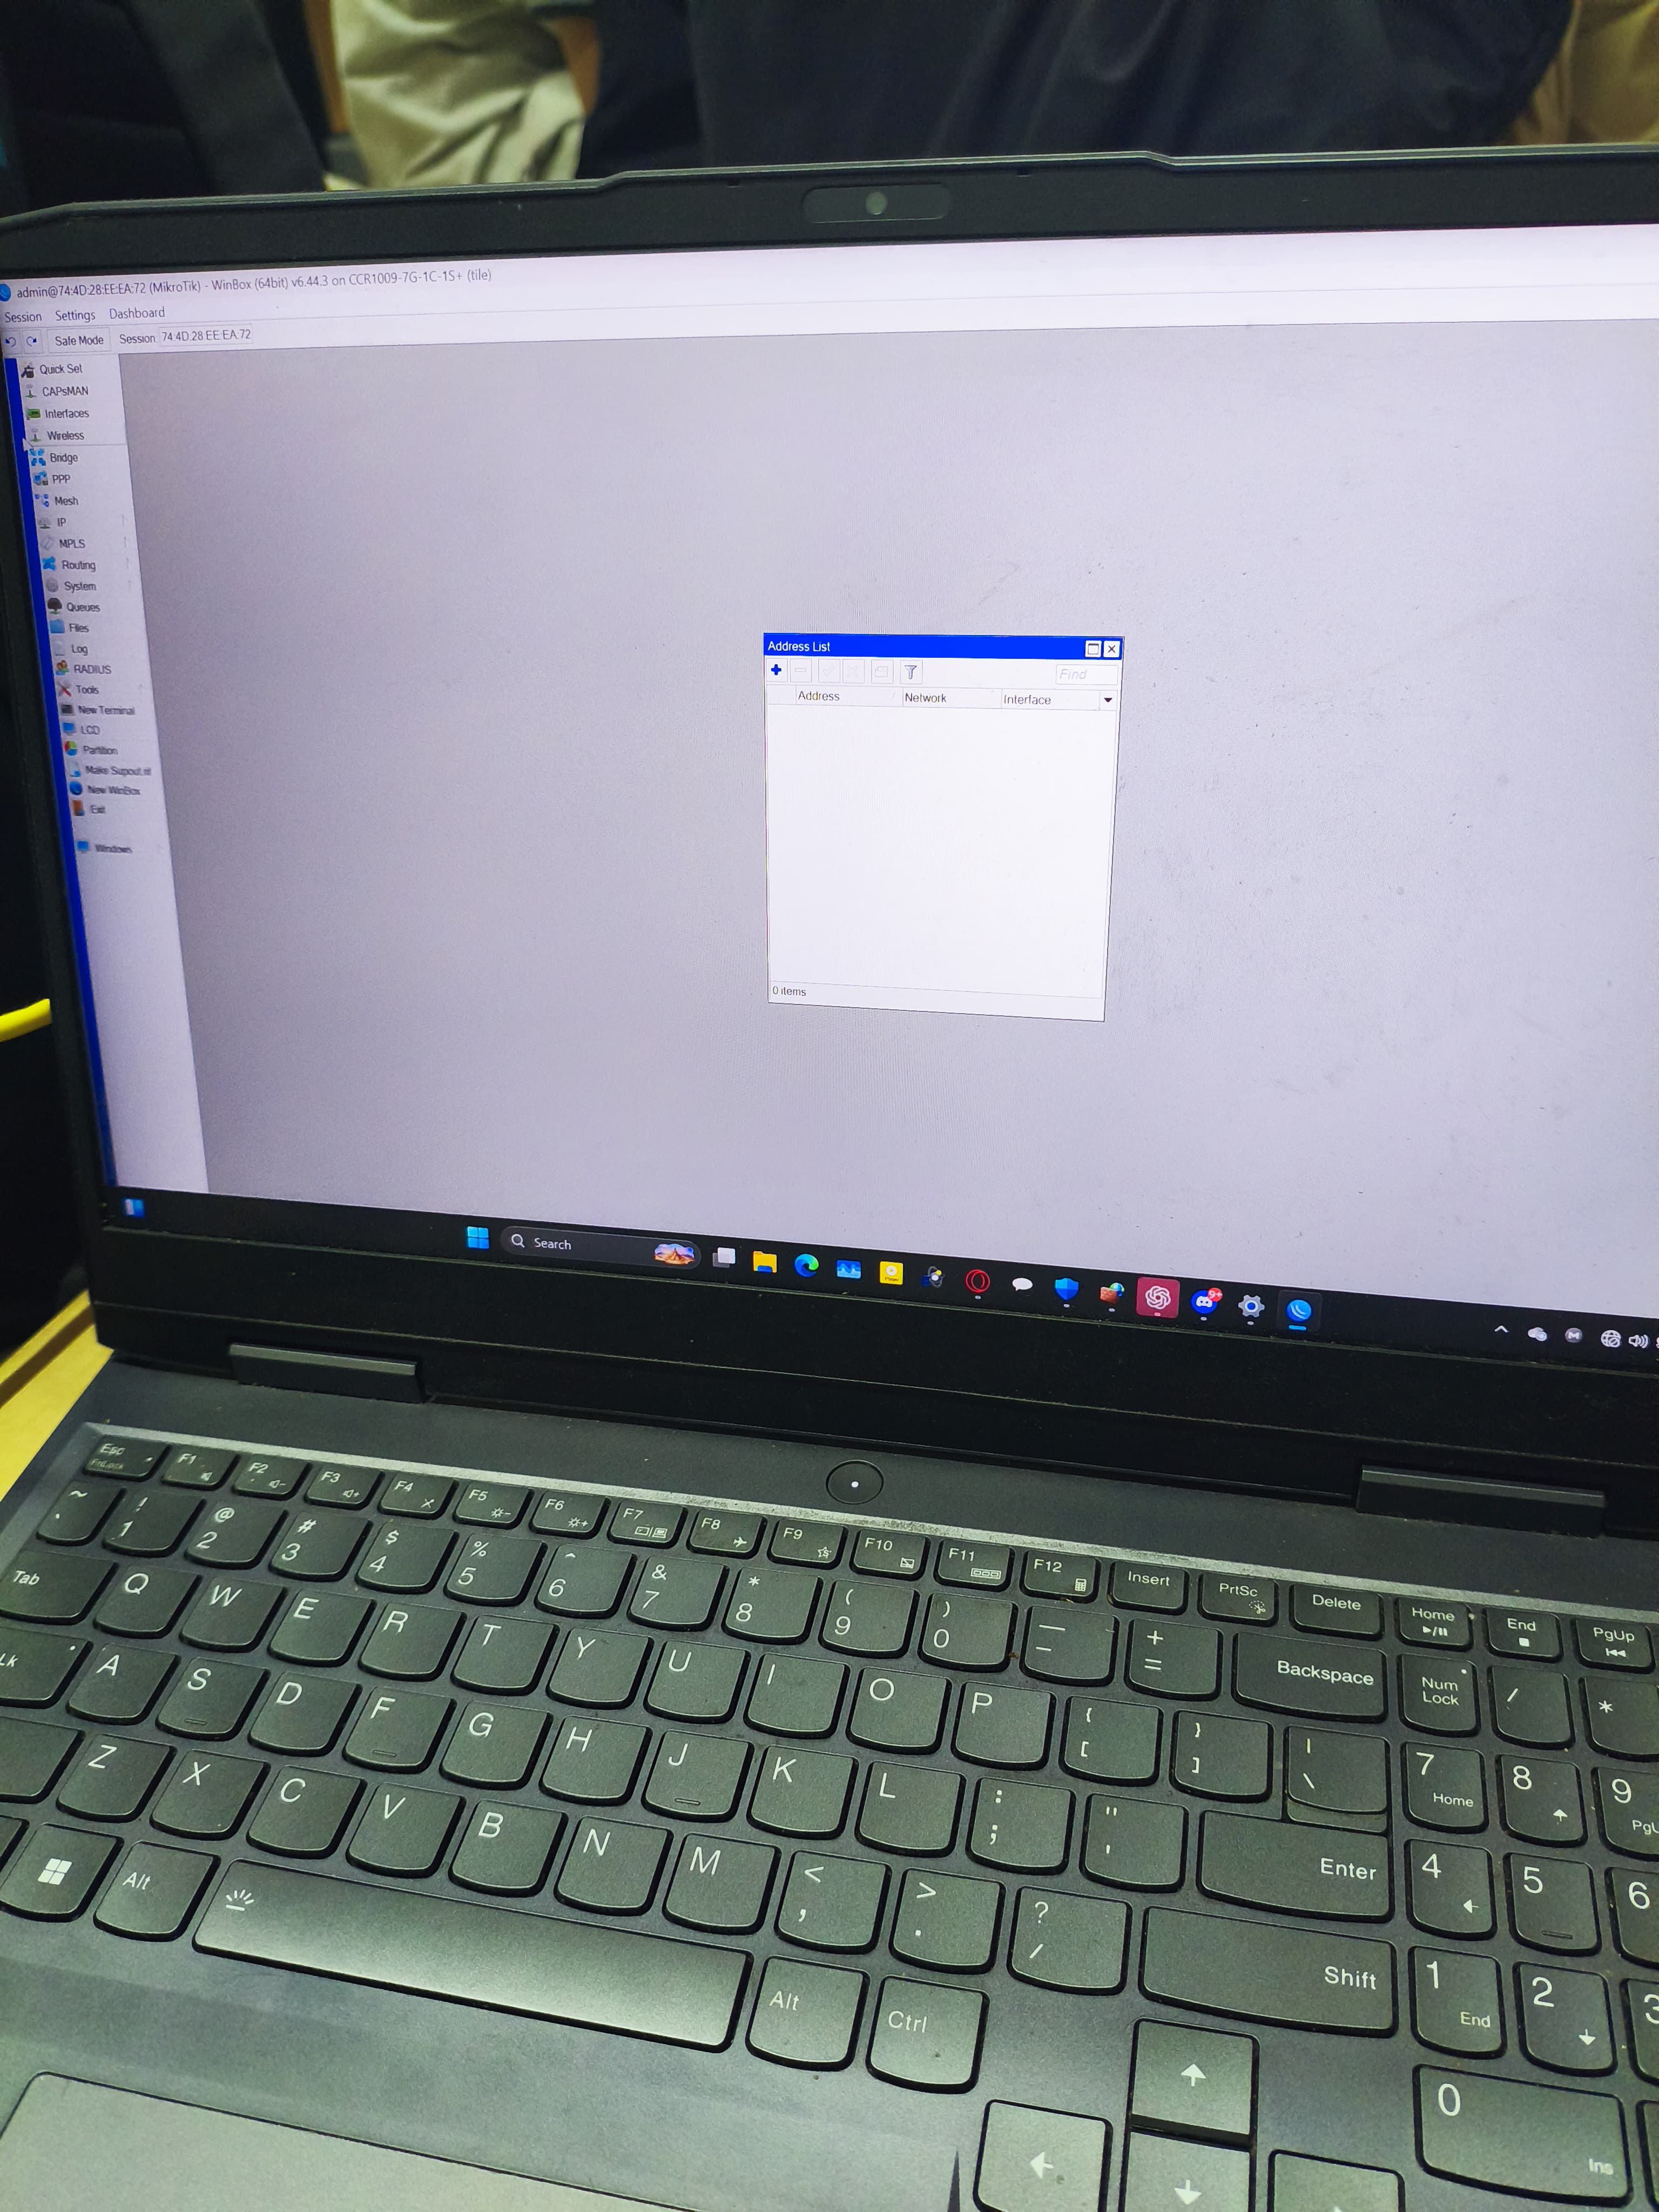
\includegraphics[width=0.5\linewidth]{P1/img/6.jpeg}
    \caption{Tampilan program Mikrotik}
    \label{fig:inirujukan}
  \end{figure}